% Options for packages loaded elsewhere
\PassOptionsToPackage{unicode}{hyperref}
\PassOptionsToPackage{hyphens}{url}
%
\documentclass[
]{article}
\usepackage{lmodern}
\usepackage{amssymb,amsmath}
\usepackage{ifxetex,ifluatex}
\ifnum 0\ifxetex 1\fi\ifluatex 1\fi=0 % if pdftex
  \usepackage[T1]{fontenc}
  \usepackage[utf8]{inputenc}
  \usepackage{textcomp} % provide euro and other symbols
\else % if luatex or xetex
  \usepackage{unicode-math}
  \defaultfontfeatures{Scale=MatchLowercase}
  \defaultfontfeatures[\rmfamily]{Ligatures=TeX,Scale=1}
\fi
% Use upquote if available, for straight quotes in verbatim environments
\IfFileExists{upquote.sty}{\usepackage{upquote}}{}
\IfFileExists{microtype.sty}{% use microtype if available
  \usepackage[]{microtype}
  \UseMicrotypeSet[protrusion]{basicmath} % disable protrusion for tt fonts
}{}
\makeatletter
\@ifundefined{KOMAClassName}{% if non-KOMA class
  \IfFileExists{parskip.sty}{%
    \usepackage{parskip}
  }{% else
    \setlength{\parindent}{0pt}
    \setlength{\parskip}{6pt plus 2pt minus 1pt}}
}{% if KOMA class
  \KOMAoptions{parskip=half}}
\makeatother
\usepackage{xcolor}
\IfFileExists{xurl.sty}{\usepackage{xurl}}{} % add URL line breaks if available
\IfFileExists{bookmark.sty}{\usepackage{bookmark}}{\usepackage{hyperref}}
\hypersetup{
  pdftitle={Results of PangoVis},
  pdfauthor={Devan Becker},
  hidelinks,
  pdfcreator={LaTeX via pandoc}}
\urlstyle{same} % disable monospaced font for URLs
\usepackage[margin=1in]{geometry}
\usepackage{color}
\usepackage{fancyvrb}
\newcommand{\VerbBar}{|}
\newcommand{\VERB}{\Verb[commandchars=\\\{\}]}
\DefineVerbatimEnvironment{Highlighting}{Verbatim}{commandchars=\\\{\}}
% Add ',fontsize=\small' for more characters per line
\usepackage{framed}
\definecolor{shadecolor}{RGB}{248,248,248}
\newenvironment{Shaded}{\begin{snugshade}}{\end{snugshade}}
\newcommand{\AlertTok}[1]{\textcolor[rgb]{0.94,0.16,0.16}{#1}}
\newcommand{\AnnotationTok}[1]{\textcolor[rgb]{0.56,0.35,0.01}{\textbf{\textit{#1}}}}
\newcommand{\AttributeTok}[1]{\textcolor[rgb]{0.77,0.63,0.00}{#1}}
\newcommand{\BaseNTok}[1]{\textcolor[rgb]{0.00,0.00,0.81}{#1}}
\newcommand{\BuiltInTok}[1]{#1}
\newcommand{\CharTok}[1]{\textcolor[rgb]{0.31,0.60,0.02}{#1}}
\newcommand{\CommentTok}[1]{\textcolor[rgb]{0.56,0.35,0.01}{\textit{#1}}}
\newcommand{\CommentVarTok}[1]{\textcolor[rgb]{0.56,0.35,0.01}{\textbf{\textit{#1}}}}
\newcommand{\ConstantTok}[1]{\textcolor[rgb]{0.00,0.00,0.00}{#1}}
\newcommand{\ControlFlowTok}[1]{\textcolor[rgb]{0.13,0.29,0.53}{\textbf{#1}}}
\newcommand{\DataTypeTok}[1]{\textcolor[rgb]{0.13,0.29,0.53}{#1}}
\newcommand{\DecValTok}[1]{\textcolor[rgb]{0.00,0.00,0.81}{#1}}
\newcommand{\DocumentationTok}[1]{\textcolor[rgb]{0.56,0.35,0.01}{\textbf{\textit{#1}}}}
\newcommand{\ErrorTok}[1]{\textcolor[rgb]{0.64,0.00,0.00}{\textbf{#1}}}
\newcommand{\ExtensionTok}[1]{#1}
\newcommand{\FloatTok}[1]{\textcolor[rgb]{0.00,0.00,0.81}{#1}}
\newcommand{\FunctionTok}[1]{\textcolor[rgb]{0.00,0.00,0.00}{#1}}
\newcommand{\ImportTok}[1]{#1}
\newcommand{\InformationTok}[1]{\textcolor[rgb]{0.56,0.35,0.01}{\textbf{\textit{#1}}}}
\newcommand{\KeywordTok}[1]{\textcolor[rgb]{0.13,0.29,0.53}{\textbf{#1}}}
\newcommand{\NormalTok}[1]{#1}
\newcommand{\OperatorTok}[1]{\textcolor[rgb]{0.81,0.36,0.00}{\textbf{#1}}}
\newcommand{\OtherTok}[1]{\textcolor[rgb]{0.56,0.35,0.01}{#1}}
\newcommand{\PreprocessorTok}[1]{\textcolor[rgb]{0.56,0.35,0.01}{\textit{#1}}}
\newcommand{\RegionMarkerTok}[1]{#1}
\newcommand{\SpecialCharTok}[1]{\textcolor[rgb]{0.00,0.00,0.00}{#1}}
\newcommand{\SpecialStringTok}[1]{\textcolor[rgb]{0.31,0.60,0.02}{#1}}
\newcommand{\StringTok}[1]{\textcolor[rgb]{0.31,0.60,0.02}{#1}}
\newcommand{\VariableTok}[1]{\textcolor[rgb]{0.00,0.00,0.00}{#1}}
\newcommand{\VerbatimStringTok}[1]{\textcolor[rgb]{0.31,0.60,0.02}{#1}}
\newcommand{\WarningTok}[1]{\textcolor[rgb]{0.56,0.35,0.01}{\textbf{\textit{#1}}}}
\usepackage{longtable,booktabs}
% Correct order of tables after \paragraph or \subparagraph
\usepackage{etoolbox}
\makeatletter
\patchcmd\longtable{\par}{\if@noskipsec\mbox{}\fi\par}{}{}
\makeatother
% Allow footnotes in longtable head/foot
\IfFileExists{footnotehyper.sty}{\usepackage{footnotehyper}}{\usepackage{footnote}}
\makesavenoteenv{longtable}
\usepackage{graphicx}
\makeatletter
\def\maxwidth{\ifdim\Gin@nat@width>\linewidth\linewidth\else\Gin@nat@width\fi}
\def\maxheight{\ifdim\Gin@nat@height>\textheight\textheight\else\Gin@nat@height\fi}
\makeatother
% Scale images if necessary, so that they will not overflow the page
% margins by default, and it is still possible to overwrite the defaults
% using explicit options in \includegraphics[width, height, ...]{}
\setkeys{Gin}{width=\maxwidth,height=\maxheight,keepaspectratio}
% Set default figure placement to htbp
\makeatletter
\def\fps@figure{htbp}
\makeatother
\setlength{\emergencystretch}{3em} % prevent overfull lines
\providecommand{\tightlist}{%
  \setlength{\itemsep}{0pt}\setlength{\parskip}{0pt}}
\setcounter{secnumdepth}{-\maxdimen} % remove section numbering
\usepackage[]{natbib}
\bibliographystyle{plainnat}

\title{Results of PangoVis}
\author{Devan Becker}
\date{2021-08-25}

\begin{document}
\maketitle

\hypertarget{load-packages-and-data}{%
\section{Load Packages and Data}\label{load-packages-and-data}}

\begin{Shaded}
\begin{Highlighting}[]
\CommentTok{\# Packages that Art hates}
\KeywordTok{library}\NormalTok{(dplyr)}
\end{Highlighting}
\end{Shaded}

\begin{verbatim}
## 
## Attaching package: 'dplyr'
\end{verbatim}

\begin{verbatim}
## The following objects are masked from 'package:stats':
## 
##     filter, lag
\end{verbatim}

\begin{verbatim}
## The following objects are masked from 'package:base':
## 
##     intersect, setdiff, setequal, union
\end{verbatim}

\begin{Shaded}
\begin{Highlighting}[]
\KeywordTok{library}\NormalTok{(tidyr)}
\KeywordTok{library}\NormalTok{(ggplot2)}
\KeywordTok{library}\NormalTok{(stringr)}
\KeywordTok{library}\NormalTok{(here)}
\end{Highlighting}
\end{Shaded}

\begin{verbatim}
## here() starts at /mnt/BCC20BCCC20B8A3A/sup
\end{verbatim}

\begin{Shaded}
\begin{Highlighting}[]
\NormalTok{dirich \textless{}{-}}\StringTok{ }\NormalTok{params}\OperatorTok{$}\NormalTok{dirich}

\CommentTok{\# Read in CSV files}
\NormalTok{csvs \textless{}{-}}\StringTok{ }\KeywordTok{list.files}\NormalTok{(}\KeywordTok{here}\NormalTok{(}\StringTok{"data/"}\NormalTok{, }\StringTok{"pangolineages"}\NormalTok{),}
    \DataTypeTok{pattern =} \KeywordTok{ifelse}\NormalTok{(dirich, }\StringTok{"*\_d.csv"}\NormalTok{, }\StringTok{"*.csv"}\NormalTok{),}
    \DataTypeTok{full.names =} \OtherTok{TRUE}\NormalTok{)}

\CommentTok{\# Remove any copies}
\NormalTok{csvs \textless{}{-}}\StringTok{ }\NormalTok{csvs[}\OperatorTok{!}\KeywordTok{grepl}\NormalTok{(}\StringTok{"{-}1"}\NormalTok{, csvs)]}

\CommentTok{\# Bring them into one data frame}
\NormalTok{lins \textless{}{-}}\StringTok{ }\KeywordTok{bind\_rows}\NormalTok{(}\KeywordTok{lapply}\NormalTok{(csvs, read.csv))}

\CommentTok{\# Taxon is encoded as \_ACCSESSIONNUMBER.ID, split into ACCESSIONNUMBER and ID}
\NormalTok{lins \textless{}{-}}\StringTok{ }\NormalTok{lins }\OperatorTok{\%\textgreater{}\%}
\StringTok{    }\KeywordTok{separate}\NormalTok{(}\DataTypeTok{col =} \StringTok{"taxon"}\NormalTok{, }\DataTypeTok{sep =} \StringTok{"}\CharTok{\textbackslash{}\textbackslash{}}\StringTok{."}\NormalTok{,}
        \DataTypeTok{into =} \KeywordTok{c}\NormalTok{(}\StringTok{"taxon"}\NormalTok{, }\StringTok{"sample"}\NormalTok{)) }\OperatorTok{\%\textgreater{}\%}
\StringTok{    }\KeywordTok{mutate}\NormalTok{(}\DataTypeTok{taxon =} \KeywordTok{str\_replace}\NormalTok{(taxon, }\StringTok{"}\CharTok{\textbackslash{}\textbackslash{}}\StringTok{\_"}\NormalTok{, }\StringTok{""}\NormalTok{))}

\NormalTok{badlins \textless{}{-}}\StringTok{ }\KeywordTok{table}\NormalTok{(lins}\OperatorTok{$}\NormalTok{taxon)}
\NormalTok{badlins \textless{}{-}}\StringTok{ }\KeywordTok{names}\NormalTok{(badlins[}\KeywordTok{which}\NormalTok{(badlins }\OperatorTok{\textless{}}\StringTok{ }\DecValTok{4500}\NormalTok{)])}
\KeywordTok{cat}\NormalTok{(}\KeywordTok{length}\NormalTok{(badlins), }\StringTok{" runs were removed for having too few samples."}\NormalTok{)}
\end{Highlighting}
\end{Shaded}

\begin{verbatim}
## 0  runs were removed for having too few samples.
\end{verbatim}

\begin{Shaded}
\begin{Highlighting}[]
\NormalTok{lins \textless{}{-}}\StringTok{ }\KeywordTok{filter}\NormalTok{(lins, }\OperatorTok{!}\NormalTok{taxon }\OperatorTok{\%in\%}\StringTok{ }\NormalTok{badlins)}

\KeywordTok{write.csv}\NormalTok{(lins, }\KeywordTok{here}\NormalTok{(}\StringTok{"data"}\NormalTok{, }\StringTok{"output"}\NormalTok{, }\StringTok{"lins.csv"}\NormalTok{),}
    \DataTypeTok{row.names =} \OtherTok{FALSE}\NormalTok{)}

\CommentTok{\#\#\#\# Visualize the uncertainty in the base calls {-}{-}{-}{-}}
\NormalTok{taxons \textless{}{-}}\StringTok{ }\KeywordTok{sort}\NormalTok{(}\KeywordTok{unique}\NormalTok{(lins}\OperatorTok{$}\NormalTok{taxon))}
\KeywordTok{length}\NormalTok{(taxons)}
\end{Highlighting}
\end{Shaded}

\begin{verbatim}
## [1] 118
\end{verbatim}

\hypertarget{abstract-info}{%
\section{Abstract Info}\label{abstract-info}}

\begin{Shaded}
\begin{Highlighting}[]
\NormalTok{summs \textless{}{-}}\StringTok{ }\NormalTok{lins }\OperatorTok{\%\textgreater{}\%}
\StringTok{    }\KeywordTok{group\_by}\NormalTok{(taxon) }\OperatorTok{\%\textgreater{}\%}
\StringTok{    }\KeywordTok{summarise}\NormalTok{(}
        \DataTypeTok{maxperc =} \KeywordTok{mean}\NormalTok{(lineage }\OperatorTok{==}\StringTok{ }\KeywordTok{names}\NormalTok{(}\KeywordTok{sort}\NormalTok{(}\KeywordTok{table}\NormalTok{(lineage),}
            \DataTypeTok{decreasing =} \OtherTok{TRUE}\NormalTok{)[}\DecValTok{1}\NormalTok{])),}
        \DataTypeTok{uniques =} \KeywordTok{length}\NormalTok{(}\KeywordTok{unique}\NormalTok{(lineage)),}
        \DataTypeTok{minpango =} \KeywordTok{min}\NormalTok{(probability),}
        \DataTypeTok{maxpango =} \KeywordTok{max}\NormalTok{(probability),}
        \DataTypeTok{menpango =} \KeywordTok{mean}\NormalTok{(probability),}
        \DataTypeTok{max =} \KeywordTok{names}\NormalTok{(}\KeywordTok{sort}\NormalTok{(}\KeywordTok{table}\NormalTok{(lineage), }\DataTypeTok{decreasing =} \OtherTok{TRUE}\NormalTok{))[}\DecValTok{1}\NormalTok{])}

\KeywordTok{print}\NormalTok{(}\StringTok{"summary info"}\NormalTok{)}
\KeywordTok{print}\NormalTok{(summs)}
\DecValTok{1} \OperatorTok{{-}}\StringTok{ }\KeywordTok{mean}\NormalTok{(summs}\OperatorTok{$}\NormalTok{maxperc); }\DecValTok{1} \OperatorTok{{-}}\StringTok{ }\KeywordTok{mean}\NormalTok{(summs}\OperatorTok{$}\NormalTok{menpango)}
\end{Highlighting}
\end{Shaded}

\hypertarget{stacked-bar-plots}{%
\section{Stacked Bar Plots}\label{stacked-bar-plots}}

\scriptsize

\begin{Shaded}
\begin{Highlighting}[]
\NormalTok{max\_label \textless{}{-}}\StringTok{ }\DecValTok{250}
\NormalTok{other\_label \textless{}{-}}\StringTok{ }\DecValTok{100}

\KeywordTok{par}\NormalTok{(}\DataTypeTok{mfrow =} \KeywordTok{c}\NormalTok{(}\DecValTok{17}\NormalTok{, }\DecValTok{1}\NormalTok{), }\DataTypeTok{mar =} \KeywordTok{c}\NormalTok{(}\FloatTok{0.05}\NormalTok{, }\FloatTok{7.75}\NormalTok{, }\FloatTok{0.05}\NormalTok{, }\FloatTok{0.05}\NormalTok{))}
\ControlFlowTok{if}\NormalTok{ (}\KeywordTok{exists}\NormalTok{(}\StringTok{"seq\_info"}\NormalTok{)) }\KeywordTok{rm}\NormalTok{(seq\_info)}
\ControlFlowTok{for}\NormalTok{ (i }\ControlFlowTok{in} \KeywordTok{seq\_along}\NormalTok{(taxons)) \{}
\NormalTok{    pang \textless{}{-}}\StringTok{ }\NormalTok{lins[lins}\OperatorTok{$}\NormalTok{taxon }\OperatorTok{==}\StringTok{ }\NormalTok{taxons[i], ]}
\NormalTok{    called \textless{}{-}}\StringTok{ }\NormalTok{pang}\OperatorTok{$}\NormalTok{lineage[pang}\OperatorTok{$}\NormalTok{sample }\OperatorTok{==}\StringTok{ }\DecValTok{0}\NormalTok{][}\DecValTok{1}\NormalTok{]}
\NormalTok{    pangtab \textless{}{-}}\StringTok{ }\KeywordTok{sort}\NormalTok{(}\KeywordTok{table}\NormalTok{(pang}\OperatorTok{$}\NormalTok{lineage), }\DataTypeTok{decreasing =} \OtherTok{TRUE}\NormalTok{)}

    \CommentTok{\# Prep the data for a nicely formatted table}
    \CommentTok{\# Subtract one because of the conseq.}
\NormalTok{    seq\_info\_i \textless{}{-}}\StringTok{ }\KeywordTok{data.frame}\NormalTok{(}
        \DataTypeTok{called =}\NormalTok{ called,}
        \DataTypeTok{mode =} \KeywordTok{names}\NormalTok{(pangtab)[}\DecValTok{1}\NormalTok{],}
            \DataTypeTok{mode\_n =}\NormalTok{ pangtab[}\DecValTok{1}\NormalTok{] }\OperatorTok{{-}}\StringTok{ }\DecValTok{1}\NormalTok{,}
            \DataTypeTok{perc =} \KeywordTok{round}\NormalTok{(}\DecValTok{100} \OperatorTok{*}\StringTok{ }\NormalTok{(pangtab[}\DecValTok{1}\NormalTok{] }\OperatorTok{{-}}\StringTok{ }\DecValTok{1}\NormalTok{) }\OperatorTok{/}\StringTok{ }\NormalTok{(}\KeywordTok{sum}\NormalTok{(pangtab) }\OperatorTok{{-}}\StringTok{ }\DecValTok{1}\NormalTok{), }\DecValTok{2}\NormalTok{),}
        \DataTypeTok{runner\_up =} \KeywordTok{names}\NormalTok{(pangtab)[}\DecValTok{2}\NormalTok{],}
            \DataTypeTok{ru\_n =}\NormalTok{ pangtab[}\DecValTok{2}\NormalTok{],}
        \DataTypeTok{unique =} \KeywordTok{length}\NormalTok{(pangtab), }\DataTypeTok{atoms =} \KeywordTok{sum}\NormalTok{(pangtab }\OperatorTok{==}\StringTok{ }\DecValTok{1}\NormalTok{))}
\NormalTok{    seq\_info\_i}\OperatorTok{$}\NormalTok{taxon \textless{}{-}}\StringTok{ }\NormalTok{taxons[i]}

    \ControlFlowTok{if}\NormalTok{ (}\OperatorTok{!}\KeywordTok{exists}\NormalTok{(}\StringTok{"seq\_info"}\NormalTok{)) \{}
\NormalTok{        seq\_info \textless{}{-}}\StringTok{ }\NormalTok{seq\_info\_i}
\NormalTok{    \} }\ControlFlowTok{else}\NormalTok{ \{}
\NormalTok{        seq\_info \textless{}{-}}\StringTok{ }\KeywordTok{bind\_rows}\NormalTok{(seq\_info, seq\_info\_i)}
\NormalTok{    \}}

\NormalTok{    colvec \textless{}{-}}\StringTok{ }\KeywordTok{rep}\NormalTok{(}\StringTok{"grey"}\NormalTok{, }\KeywordTok{length}\NormalTok{(pangtab))}
\NormalTok{    colvec[}\KeywordTok{which}\NormalTok{(}\KeywordTok{names}\NormalTok{(pangtab) }\OperatorTok{==}\StringTok{ }\NormalTok{called)] \textless{}{-}}\StringTok{ "red"}

\NormalTok{    n \textless{}{-}}\StringTok{ }\KeywordTok{sum}\NormalTok{(pangtab }\OperatorTok{\textgreater{}}\StringTok{ }\NormalTok{max\_label)}
    \ControlFlowTok{if}\NormalTok{ (n }\OperatorTok{\textgreater{}}\StringTok{ }\DecValTok{1}\NormalTok{) \{}
\NormalTok{        add\_other \textless{}{-}}\StringTok{ }\OtherTok{FALSE}
        \ControlFlowTok{if}\NormalTok{ (}\KeywordTok{sum}\NormalTok{(pangtab }\OperatorTok{\textless{}}\StringTok{ }\NormalTok{other\_label) }\OperatorTok{\textgreater{}}\StringTok{ }\DecValTok{10}\NormalTok{) \{}
\NormalTok{            add\_other \textless{}{-}}\StringTok{ }\OtherTok{TRUE}
\NormalTok{            other\_count \textless{}{-}}\StringTok{ }\KeywordTok{sum}\NormalTok{(pangtab }\OperatorTok{\textless{}=}\StringTok{ }\NormalTok{other\_label)}
\NormalTok{            pangtab \textless{}{-}}\StringTok{ }\KeywordTok{c}\NormalTok{(pangtab[pangtab }\OperatorTok{\textgreater{}}\StringTok{ }\NormalTok{other\_label],}
                \KeywordTok{c}\NormalTok{(}\StringTok{"other"}\NormalTok{ =}\StringTok{ }\KeywordTok{sum}\NormalTok{(pangtab[pangtab }\OperatorTok{\textless{}=}\StringTok{ }\NormalTok{other\_label])))}
\NormalTok{            colvec[}\KeywordTok{which}\NormalTok{(}\KeywordTok{names}\NormalTok{(pangtab) }\OperatorTok{==}\StringTok{ "other"}\NormalTok{)] \textless{}{-}}\StringTok{ "black"}
\NormalTok{        \}}
\NormalTok{        barlabx \textless{}{-}}\StringTok{ }\KeywordTok{c}\NormalTok{(}\DecValTok{0}\NormalTok{, }\KeywordTok{cumsum}\NormalTok{(pangtab[}\DecValTok{1}\OperatorTok{:}\NormalTok{(n }\OperatorTok{{-}}\StringTok{ }\DecValTok{1}\NormalTok{)])) }\OperatorTok{+}
\StringTok{            }\NormalTok{pangtab[}\DecValTok{1}\OperatorTok{:}\NormalTok{n] }\OperatorTok{/}\StringTok{ }\DecValTok{2}
\NormalTok{        barlabels \textless{}{-}}\StringTok{ }\KeywordTok{names}\NormalTok{(pangtab)[}\DecValTok{1}\OperatorTok{:}\NormalTok{n]}
\NormalTok{        barlens \textless{}{-}}\StringTok{ }\KeywordTok{sapply}\NormalTok{(}\KeywordTok{gregexpr}\NormalTok{(}\StringTok{"}\CharTok{\textbackslash{}\textbackslash{}}\StringTok{."}\NormalTok{, barlabels), length)}
        \ControlFlowTok{for}\NormalTok{ (j }\ControlFlowTok{in} \KeywordTok{seq\_along}\NormalTok{(barlabels)) \{}
            \ControlFlowTok{if}\NormalTok{ (pangtab[j] }\OperatorTok{\textless{}}\StringTok{ }\DecValTok{400} \OperatorTok{\&}\StringTok{ }\NormalTok{barlens[j] }\OperatorTok{\textgreater{}=}\StringTok{ }\DecValTok{2}\NormalTok{) \{}
\NormalTok{                barsplit \textless{}{-}}\StringTok{ }\KeywordTok{strsplit}\NormalTok{(barlabels[j], }\DataTypeTok{split =} \StringTok{"}\CharTok{\textbackslash{}\textbackslash{}}\StringTok{."}\NormalTok{)[[}\DecValTok{1}\NormalTok{]]}
\NormalTok{                barn \textless{}{-}}\StringTok{ }\KeywordTok{length}\NormalTok{(barsplit)}
\NormalTok{                half \textless{}{-}}\StringTok{ }\KeywordTok{floor}\NormalTok{(barn }\OperatorTok{/}\StringTok{ }\DecValTok{2}\NormalTok{)}
\NormalTok{                barlabels[j] \textless{}{-}}\StringTok{ }\KeywordTok{paste0}\NormalTok{(}
                    \KeywordTok{paste}\NormalTok{(barsplit[}\DecValTok{1}\OperatorTok{:}\NormalTok{half], }\DataTypeTok{collapse =} \StringTok{"."}\NormalTok{),}
                    \StringTok{".}\CharTok{\textbackslash{}n}\StringTok{"}\NormalTok{,}
                    \KeywordTok{paste}\NormalTok{(barsplit[(half }\OperatorTok{+}\StringTok{ }\DecValTok{1}\NormalTok{)}\OperatorTok{:}\NormalTok{barn], }\DataTypeTok{collapse =} \StringTok{"."}\NormalTok{)}
\NormalTok{                )}
\NormalTok{            \}}
\NormalTok{        \}}

        \KeywordTok{barplot}\NormalTok{(}\KeywordTok{as.matrix}\NormalTok{(pangtab),}
            \DataTypeTok{col =}\NormalTok{ colvec, }\DataTypeTok{hori =} \OtherTok{TRUE}\NormalTok{, }\DataTypeTok{axes =} \OtherTok{FALSE}\NormalTok{)}
        \KeywordTok{text}\NormalTok{(barlabx, }\FloatTok{0.7}\NormalTok{, barlabels, }\DataTypeTok{cex =} \FloatTok{1.5}\NormalTok{)}
        \ControlFlowTok{if}\NormalTok{ (add\_other) \{}
            \KeywordTok{text}\NormalTok{(}\DataTypeTok{x =} \KeywordTok{sum}\NormalTok{(pangtab) }\OperatorTok{{-}}\StringTok{ }\NormalTok{pangtab[}\StringTok{"other"}\NormalTok{] }\OperatorTok{/}\StringTok{ }\DecValTok{2}\NormalTok{,}
            \DataTypeTok{y =} \FloatTok{0.7}\NormalTok{, }\DataTypeTok{col =} \StringTok{"white"}\NormalTok{, }\DataTypeTok{cex =} \FloatTok{1.5}\NormalTok{,}
            \DataTypeTok{label =} \KeywordTok{paste0}\NormalTok{(}\StringTok{"Others:}\CharTok{\textbackslash{}n}\StringTok{"}\NormalTok{, other\_count))}
\NormalTok{        \}}
        \KeywordTok{mtext}\NormalTok{(}\DataTypeTok{side =} \DecValTok{2}\NormalTok{, }\DataTypeTok{cex =} \DecValTok{1}\NormalTok{, }\DataTypeTok{las =} \DecValTok{1}\NormalTok{,}
            \DataTypeTok{text =} \KeywordTok{paste}\NormalTok{(}\KeywordTok{substr}\NormalTok{(taxons[i], }\DecValTok{1}\NormalTok{, }\DecValTok{3}\NormalTok{),}
                \KeywordTok{substr}\NormalTok{(taxons[i], }\DecValTok{4}\NormalTok{, }\DecValTok{20}\NormalTok{), }\DataTypeTok{sep =} \StringTok{"}\CharTok{\textbackslash{}n}\StringTok{"}\NormalTok{))}
        \KeywordTok{abline}\NormalTok{(}\DataTypeTok{v =} \KeywordTok{seq}\NormalTok{(}\DecValTok{0}\NormalTok{, }\DecValTok{10000}\NormalTok{, }\DecValTok{1000}\NormalTok{), }\DataTypeTok{lty =} \DecValTok{2}\NormalTok{)}
        \StringTok{"pretty\_labels \textless{}{-} seq(0, sum(pangtab),}
\StringTok{                by = ifelse(sum(pangtab) \textless{} 2000, 100, 1000))}
\StringTok{        mtext(side = 1,}
\StringTok{            at = pretty\_labels,}
\StringTok{            text = pretty\_labels,}
\StringTok{            line = 0,}
\StringTok{            cex = 0.75}
\StringTok{        )"}
\NormalTok{    \}}
\NormalTok{\}}

\NormalTok{seq\_info}\OperatorTok{$}\NormalTok{taxon \textless{}{-}}\StringTok{ }\NormalTok{taxons}
\NormalTok{seq\_info \textless{}{-}}\StringTok{ }\KeywordTok{arrange}\NormalTok{(seq\_info, mode, mode\_n) }\OperatorTok{\%\textgreater{}\%}
\StringTok{    }\KeywordTok{select}\NormalTok{(taxon, }\KeywordTok{everything}\NormalTok{())}
\NormalTok{knitr}\OperatorTok{::}\KeywordTok{kable}\NormalTok{(seq\_info, }\DataTypeTok{row.names =} \OtherTok{FALSE}\NormalTok{)}
\end{Highlighting}
\end{Shaded}

\begin{longtable}[]{@{}lllrrlrrr@{}}
\toprule
taxon & called & mode & mode\_n & perc & runner\_up & ru\_n & unique &
atoms\tabularnewline
\midrule
\endhead
SRR12749715 & A & A & 4656 & 93.19 & B.1 & 61 & 40 & 11\tabularnewline
SRR12749716 & A & A & 4692 & 93.92 & B.1 & 48 & 34 & 11\tabularnewline
ERR5082598 & AA.3 & AA.3 & 4611 & 92.29 & B.1.177.15 & 195 & 23 &
5\tabularnewline
ERR5077713 & AD.2 & AD.2 & 4921 & 98.50 & B.1 & 23 & 12 &
4\tabularnewline
ERR4890693 & AM.3 & AM.3 & 4594 & 91.95 & B.1.1 & 249 & 46 &
18\tabularnewline
ERR4890771 & AM.3 & AM.3 & 4746 & 95.00 & B.1.1 & 122 & 41 &
16\tabularnewline
ERR5079699 & AM.3 & AM.3 & 4843 & 96.94 & B.1.1 & 62 & 27 &
11\tabularnewline
ERR4891444 & B.1.1 & B.1 & 1680 & 33.63 & B.1.1 & 764 & 270 &
63\tabularnewline
ERR4693865 & B.1 & B.1 & 2418 & 48.40 & B.1.2 & 115 & 262 &
58\tabularnewline
ERR4890531 & B.1 & B.1 & 2752 & 55.08 & B.1.1 & 89 & 255 &
62\tabularnewline
ERR4891415 & B.1 & B.1 & 2879 & 57.63 & B.1.595 & 111 & 259 &
65\tabularnewline
ERR5082578 & B.1 & B.1 & 3705 & 74.16 & B.1.280 & 154 & 153 &
41\tabularnewline
ERR4693801 & B.1.1 & B.1.1 & 2578 & 51.60 & B.1 & 173 & 247 &
64\tabularnewline
ERR4891178 & B.1.1 & B.1.1 & 2790 & 55.84 & B.1.1.307 & 184 & 251 &
50\tabularnewline
ERR4891497 & B.1.1 & B.1.1 & 2801 & 56.06 & B.1.1.374 & 102 & 241 &
54\tabularnewline
ERR4890881 & B.1.1 & B.1.1 & 3276 & 65.57 & B.1.1.217 & 151 & 228 &
58\tabularnewline
ERR4890572 & B.1.1 & B.1.1 & 3577 & 71.60 & B.1.1.121 & 171 & 168 &
46\tabularnewline
ERR4890926 & B.1.1 & B.1.1 & 3994 & 79.94 & B.1.1.217 & 50 & 189 &
55\tabularnewline
ERR4891572 & B.1.1.10 & B.1.1.10 & 4759 & 95.26 & B.1.1 & 85 & 34 &
15\tabularnewline
ERR5078897 & B.1.1.240 & B.1.1.240 & 4011 & 80.28 & B.1.1 & 443 & 123 &
53\tabularnewline
ERR4694498 & B.1.1.310 & B.1.1.310 & 4027 & 80.60 & B.1.1 & 218 & 133 &
40\tabularnewline
ERR4694380 & B.1.1.37 & B.1.1.37 & 4924 & 98.56 & B.1.1.294 & 32 & 12 &
6\tabularnewline
ERR5081836 & B.1.1.434 & B.1.1.434 & 4785 & 95.78 & B.1.1 & 68 & 32 &
21\tabularnewline
ERR4891493 & B.1.1.51 & B.1.1.51 & 4725 & 94.58 & B.1.1 & 190 & 52 &
35\tabularnewline
ERR4694330 & B.1.1.58 & B.1.1.58 & 3838 & 76.82 & B.1.1.217 & 367 & 59 &
20\tabularnewline
ERR5077924 & B.1.1.7 & B.1.1.7 & 4996 & 100.00 & NA & NA & 1 &
0\tabularnewline
ERR5078863 & B.1.1.7 & B.1.1.7 & 4996 & 100.00 & NA & NA & 1 &
0\tabularnewline
ERR5079000 & B.1.1.7 & B.1.1.7 & 4996 & 100.00 & NA & NA & 1 &
0\tabularnewline
ERR5080131 & B.1.1.7 & B.1.1.7 & 4996 & 100.00 & NA & NA & 1 &
0\tabularnewline
ERR5080504 & B.1.1.7 & B.1.1.7 & 4996 & 100.00 & NA & NA & 1 &
0\tabularnewline
ERR5082214 & B.1.1.7 & B.1.1.7 & 4996 & 100.00 & NA & NA & 1 &
0\tabularnewline
ERR5082673 & B.1.1.7 & B.1.1.7 & 4996 & 100.00 & NA & NA & 1 &
0\tabularnewline
ERR4694010 & B.1.13 & B.1.13 & 4043 & 80.92 & B.1 & 520 & 54 &
25\tabularnewline
ERR5082710 & B.1.160 & B.1.160 & 3871 & 77.48 & B.1.160.15 & 191 & 49 &
12\tabularnewline
ERR5082346 & B.1.160 & B.1.160 & 4431 & 88.69 & B.1.160.11 & 118 & 36 &
0\tabularnewline
ERR4890974 & B.1.160 & B.1.160 & 4787 & 95.82 & B.1 & 26 & 32 &
7\tabularnewline
ERR5081077 & B.1.177 & B.1.177 & 3267 & 65.39 & B.1.177.73 & 1104 & 70 &
11\tabularnewline
ERR5082706 & B.1.177 & B.1.177 & 4046 & 80.98 & B.1.177.44 & 75 & 66 &
9\tabularnewline
ERR5078210 & B.1.177 & B.1.177 & 4391 & 87.89 & B.1.177.21 & 37 & 65 &
7\tabularnewline
ERR4891001 & B.1.177 & B.1.177 & 4429 & 88.65 & B.1.177.25 & 34 & 59 &
8\tabularnewline
ERR5082656 & B.1.177 & B.1.177 & 4849 & 97.06 & B.1.177.68 & 58 & 14 &
1\tabularnewline
ERR5082694 & B.1.177 & B.1.177 & 4876 & 97.60 & B.1.177.21 & 35 & 17 &
7\tabularnewline
ERR4891304 & B.1.177 & B.1.177 & 4893 & 97.94 & B.1.177.73 & 35 & 30 &
17\tabularnewline
ERR5082606 & B.1.177 & B.1.177 & 4895 & 97.98 & B.1.177.68 & 31 & 13 &
5\tabularnewline
ERR5081293 & B.1.177 & B.1.177 & 4897 & 98.02 & B.1.258 & 27 & 15 &
7\tabularnewline
ERR4891433 & B.1.177 & B.1.177 & 4919 & 98.46 & B.1.177.68 & 28 & 11 &
5\tabularnewline
ERR4891532 & B.1.177 & B.1.177 & 4956 & 99.20 & B.1.177.68 & 18 & 9 &
1\tabularnewline
ERR4891011 & B.1.177.16 & B.1.177.16 & 4897 & 98.02 & B.1.177 & 84 & 6 &
2\tabularnewline
ERR5080327 & B.1.177.18 & B.1.177.18 & 4480 & 89.67 & B.1 & 276 & 37 &
22\tabularnewline
ERR4891061 & B.1.177.19 & B.1.177.19 & 4821 & 96.50 & B.1.2 & 50 & 14 &
5\tabularnewline
ERR4890746 & B.1.177.4 & B.1.177.4 & 4949 & 99.06 & B.1.177 & 28 & 13 &
8\tabularnewline
ERR5079423 & B.1.177.57 & B.1.177.57 & 2486 & 49.76 & B.1.177.56 & 2082
& 34 & 13\tabularnewline
ERR5082708 & B.1.177.57 & B.1.177.57 & 4922 & 98.52 & B.1.177.73 & 21 &
13 & 6\tabularnewline
ERR5082622 & B.1.177.58 & B.1.177.58 & 4898 & 98.04 & B.1.177 & 27 & 17
& 3\tabularnewline
ERR5082654 & B.1.177.65 & B.1.177.65 & 4334 & 86.75 & B.1.177 & 308 & 34
& 15\tabularnewline
ERR5082702 & B.1.177.65 & B.1.177.65 & 4802 & 96.12 & B.1.177 & 120 & 18
& 5\tabularnewline
ERR5080159 & B.1.177.7 & B.1.177.7 & 4339 & 86.85 & B.1.177.16 & 612 & 7
& 1\tabularnewline
ERR4891103 & B.1.177.9 & B.1.177.9 & 4896 & 98.00 & B.1.177 & 49 & 18 &
5\tabularnewline
ERR4891037 & B.1.258 & B.1.258 & 4729 & 94.66 & B.1.258.14 & 51 & 31 &
9\tabularnewline
ERR4891235 & B.1.258 & B.1.258 & 4827 & 96.62 & A & 26 & 26 &
4\tabularnewline
ERR4890609 & B.1.258 & B.1.258 & 4856 & 97.20 & B.1.258.14 & 40 & 23 &
7\tabularnewline
ERR4891261 & B.1.258.12 & B.1.258.12 & 4854 & 97.16 & B.1.258.14 & 27 &
17 & 3\tabularnewline
ERR5082600 & B.1.258.5 & B.1.258.5 & 4650 & 93.07 & B.1.258 & 131 & 29 &
17\tabularnewline
ERR5082700 & B.1.36.39 & B.1.36.39 & 4696 & 94.00 & B.1 & 160 & 18 &
6\tabularnewline
ERR4890820 & B.1.391 & B.1.391 & 4282 & 85.71 & B.1 & 441 & 48 &
17\tabularnewline
ERR4891675 & B.1.523 & B.1.523 & 4691 & 93.90 & B.1.400 & 135 & 27 &
12\tabularnewline
ERR4891238 & B.4.8 & B.4.8 & 4816 & 96.40 & B.1 & 56 & 25 &
10\tabularnewline
ERR4693495 & B.40 & B.40 & 4937 & 98.82 & B.1 & 23 & 11 &
3\tabularnewline
SRR12639961 & B.41 & B.41 & 3956 & 79.18 & B.1.1 & 235 & 39 &
16\tabularnewline
SRR13021017 & B.4.6 & None & 4885 & 99.53 & A & 18 & 4 &
1\tabularnewline
SRR13021008 & A.2.2 & None & 4910 & 99.63 & A & 13 & 6 &
3\tabularnewline
SRR13021020 & A & None & 4915 & 99.66 & A & 16 & 3 & 1\tabularnewline
SRR13020991 & A.1 & None & 4930 & 99.72 & A & 12 & 4 & 2\tabularnewline
SRR13021124 & B.4.6 & None & 4930 & 99.72 & A & 10 & 5 &
2\tabularnewline
SRR13021131 & B.1 & None & 4935 & 99.74 & A & 10 & 4 & 1\tabularnewline
SRR13021013 & B.1 & None & 4940 & 99.76 & A & 6 & 4 & 0\tabularnewline
SRR11433882 & B.1 & None & 4955 & 99.82 & A & 8 & 3 & 1\tabularnewline
SRR13021011 & A & None & 4960 & 99.84 & A & 8 & 2 & 0\tabularnewline
SRR11433888 & B.1.413 & None & 4965 & 99.86 & A & 5 & 4 &
2\tabularnewline
SRR11433893 & B.1 & None & 4965 & 99.86 & A & 6 & 3 & 1\tabularnewline
SRR13021109 & A.1 & None & 4970 & 99.88 & A & 4 & 3 & 0\tabularnewline
SRR13021111 & B.58 & None & 4970 & 99.88 & A & 5 & 3 & 1\tabularnewline
SRR13021113 & B.1.1 & None & 4970 & 99.88 & A & 5 & 3 & 1\tabularnewline
SRR13021099 & A.1 & None & 4980 & 99.92 & A & 2 & 3 & 0\tabularnewline
SRR13021104 & B.1.1 & None & 4985 & 99.94 & A & 2 & 3 & 1\tabularnewline
SRR13021130 & A & None & 4990 & 99.96 & A & 2 & 2 & 0\tabularnewline
SRR13020998 & B.1.1 & None & 4995 & 99.98 & B.1.1 & 1 & 2 &
1\tabularnewline
SRR13020999 & B.1 & None & 4995 & 99.98 & B.1 & 1 & 2 & 1\tabularnewline
SRR13021003 & A.1 & None & 4995 & 99.98 & A.1 & 1 & 2 & 1\tabularnewline
SRR13021010 & A.2.2 & None & 4995 & 99.98 & A.2.2 & 1 & 2 &
1\tabularnewline
SRR13021022 & A.1 & None & 4995 & 99.98 & A.1 & 1 & 2 & 1\tabularnewline
SRR13021052 & B.1.1 & None & 4995 & 99.98 & B.1.1 & 1 & 2 &
1\tabularnewline
SRR13021053 & B.1.1.71 & None & 4995 & 99.98 & B.1.1.71 & 1 & 2 &
1\tabularnewline
SRR13021059 & B.1.13 & None & 4995 & 99.98 & B.1.13 & 1 & 2 &
1\tabularnewline
SRR13021061 & A.1 & None & 4995 & 99.98 & A.1 & 1 & 2 & 1\tabularnewline
SRR13021067 & A.2.2 & None & 4995 & 99.98 & A.2.2 & 1 & 2 &
1\tabularnewline
SRR13021072 & B.1 & None & 4995 & 99.98 & B.1 & 1 & 2 & 1\tabularnewline
SRR13021073 & A.1 & None & 4995 & 99.98 & A.1 & 1 & 2 & 1\tabularnewline
SRR13021077 & A.1 & None & 4995 & 99.98 & A.1 & 1 & 2 & 1\tabularnewline
SRR13021084 & B.1 & None & 4995 & 99.98 & B.1 & 1 & 2 & 1\tabularnewline
SRR13021090 & B.1 & None & 4995 & 99.98 & B.1 & 1 & 2 & 1\tabularnewline
SRR13021093 & A.2.2 & None & 4995 & 99.98 & A.2.2 & 1 & 2 &
1\tabularnewline
SRR13021098 & A.1 & None & 4995 & 99.98 & A.1 & 1 & 2 & 1\tabularnewline
SRR13021107 & A.2.2 & None & 4995 & 99.98 & A.2.2 & 1 & 2 &
1\tabularnewline
SRR13021115 & B.1.1.10 & None & 4995 & 99.98 & B.1.1.10 & 1 & 2 &
1\tabularnewline
SRR13021133 & A & None & 4995 & 99.98 & A & 1 & 2 & 1\tabularnewline
SRR13021134 & B.4.6 & None & 4995 & 99.98 & B.4.6 & 1 & 2 &
1\tabularnewline
SRR13021135 & A.2.2 & None & 4995 & 99.98 & A.2.2 & 1 & 2 &
1\tabularnewline
SRR13021143 & A.2.2 & None & 4995 & 99.98 & A.2.2 & 1 & 2 &
1\tabularnewline
ERR4692420 & None & None & 4996 & 100.00 & NA & NA & 1 &
0\tabularnewline
ERR4692568 & None & None & 4996 & 100.00 & NA & NA & 1 &
0\tabularnewline
ERR4692877 & None & None & 4996 & 100.00 & NA & NA & 1 &
0\tabularnewline
ERR4692945 & None & None & 4996 & 100.00 & NA & NA & 1 &
0\tabularnewline
ERR4693014 & None & None & 4996 & 100.00 & NA & NA & 1 &
0\tabularnewline
ERR4693019 & None & None & 4996 & 100.00 & NA & NA & 1 &
0\tabularnewline
ERR4890819 & None & None & 4996 & 100.00 & NA & NA & 1 &
0\tabularnewline
ERR5082599 & None & None & 4996 & 100.00 & NA & NA & 1 &
0\tabularnewline
SRR13592146 & None & None & 4996 & 100.00 & NA & NA & 1 &
0\tabularnewline
\bottomrule
\end{longtable}

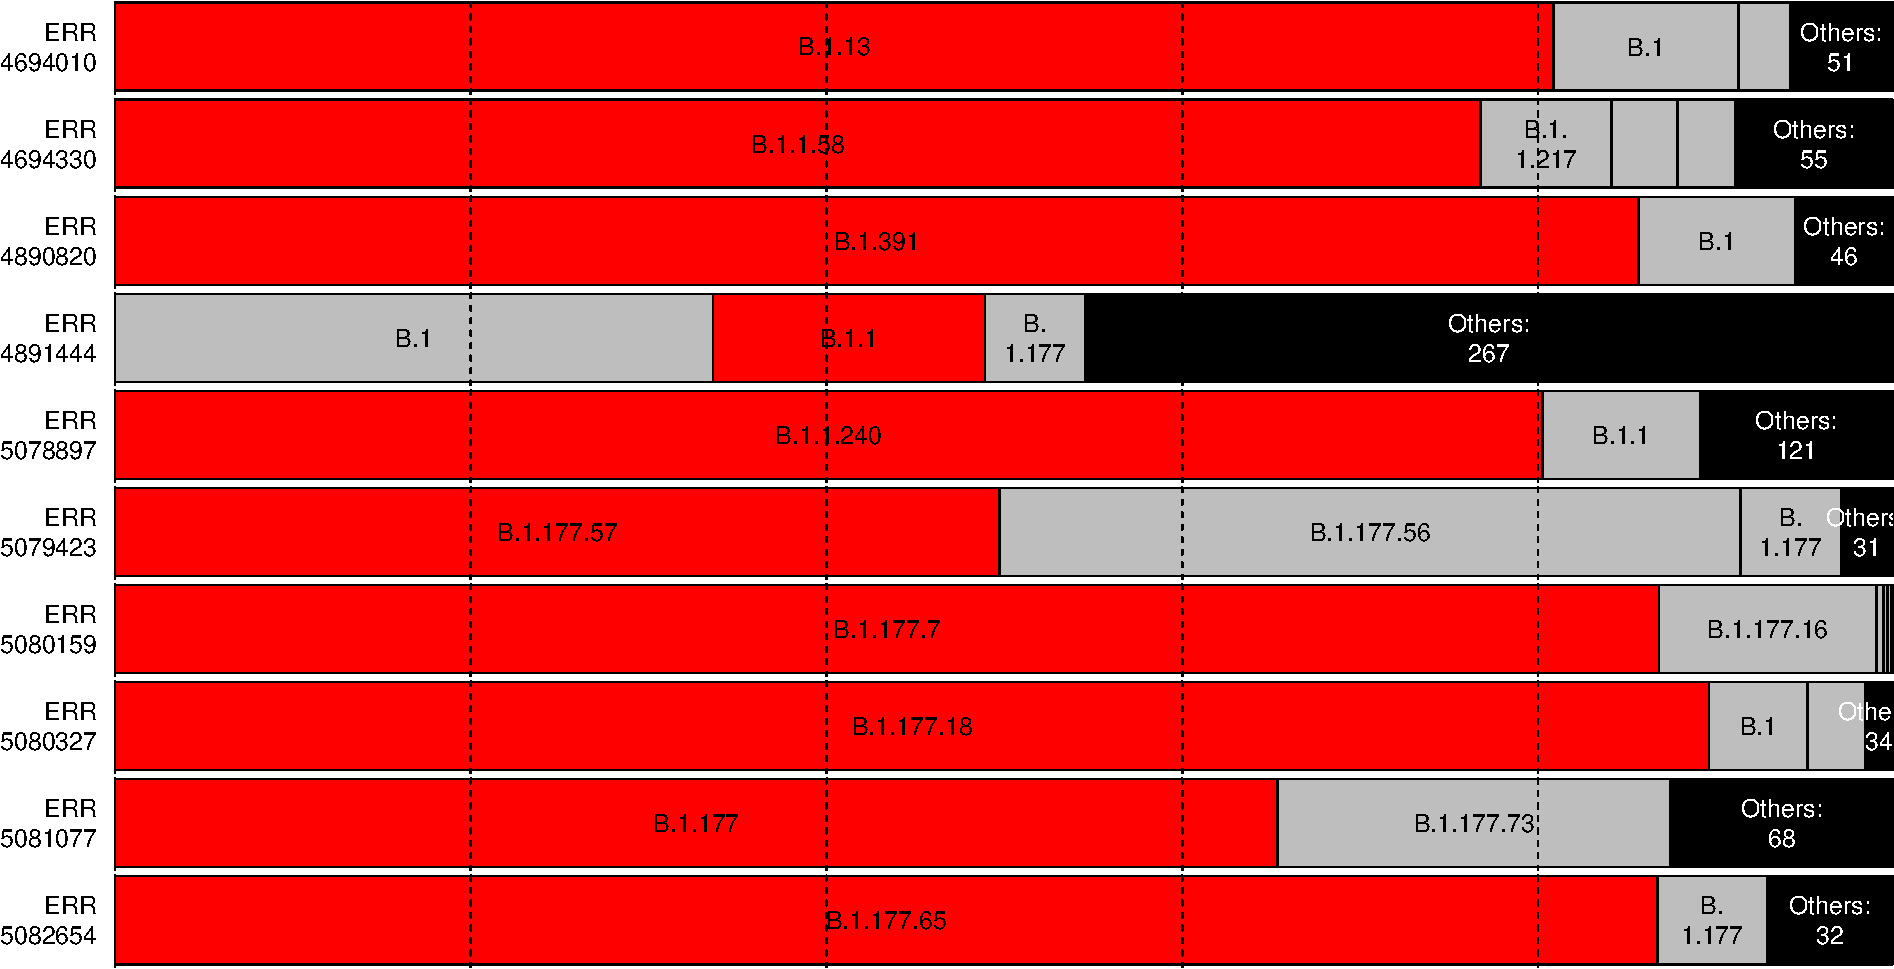
\includegraphics{pangolin_results_report_files/figure-latex/pareto-1.pdf}

\end{document}
